\section{CNNDroid}
CNNDroid is an open source deep learning library for Android. It is able to execute convolutional neural networks, supporting most CNN layers used by existing desktop/server deep learning frameworks, namely Caffe, Theano and Torch. Supported layers, as of March 2017 are:
\begin{itemize}
    \item{Convolutional Layer}
    \item{Pooling Layer}
    \item{Local Response Normalization Layer}
    \item{Fully-Connected Layer}
    \item{Rectified Linear Unit Layer (ReLU)}
    \item{Softmax Layer}
    \item{Accuracy and Top-K Layer}
\end{itemize}
Due to the library being open source, it is possible to add additional layers, such as batch normalization or sigmoid.\\
The library also supports a variety of customizations, like maximum memory usage, GPU or CPU acceleration and automatic performance tuning.

\subsection{Setup and Integration into Android Project}
CNNDroid is a source code library. That means that integration into an existing Android Project is fairly straight forward and doesn't require any third-party dependencies.\\
The only prerequisites are:
\begin{itemize}
    \item{A functional Android development environment (e.g. Android Studio\footnote{https://developer.android.com/studio/index.html})}
    \item{Android phone or emulator running at least Android SDK version 21.0 (Lollipop)}
\end{itemize}

To integrate CNNDroid into the project, the repository has to be cloned from its GitHub\footnote{https://github.com/ENCP/CNNdroid} page. Inside the \texttt{CNNdroid Source Package}' folder are three folders: \texttt{java}, \texttt{rs} and \texttt{libs}.\\
The \texttt{java} and \texttt{rs} folders need to be copied into the projects \texttt{app/src/main/} directory, merging the \texttt{java} folders.\\
The \texttt{libs} folder has to be copied and merged into the \texttt{app/} directory.\\
For effective usage of CNNDroid, it needs read and write access to storage on the smartphone. Android policies require an application to request these permissions before the app starts. These permission requests are specified inside the \texttt{AndroidManifest.xml} file. The following lines have to be added there before the \lstinline[language=XML]{<application} section:

\begin{lstlisting}[language=XML, basicstyle=\scriptsize]
    <uses-permission android:name="android.permission.READ_EXTERNAL_STORAGE"/>
    <uses-permission android:name="android.permission.WRITE_EXTERNAL_STORAGE"/>
\end{lstlisting}

To cope with the high computational requirements, CNNDroid potentially needs a large amount of memory. Therefore, the heap has to be increased, which is done by adding

\begin{lstlisting}[language=XML, basicstyle=\scriptsize]
    android::largeHeap="true"
\end{lstlisting}
\noindent
inside the \lstinline[language=XML]{<application} section.\\
Now, everything should be set up correctly and programming can commence.\\
After importing the package \lstinline[language=Java]{network.CNNdroid}, the \lstinline[language=Java]{CNNdroid} object is accessible, which can call the function \lstinline[language=Java]{CNNDroid::classify}. This is the keyword to start execution of the trained model. The specification of the model is explained in the following section.

\subsection{Structure of necessary CNNDroid Files}
Of course, CNNDroid needs to know how to classify an input. For that it either uses converted binary layer files, created by a desktop deep learning framework, or internal conversion functions (e.g. for pooling or ReLU).\\
The layer BLObs\footnote{Binary Large Objects} are generally used for more complicated layers, such as convolutional or fully connected layers, which have high dimensional variables (weight matrices). These files have to be converted into the MessagePack\footnote{http://msgpack.org/} format and put onto the smartphones storage.\\
The order in which the layers are executed, additional configurations and layers which do not need a BLOb file are defined inside the definition file. This file is used as a settings file for the \lstinline[language=Java]{CNNdroid} classifier.\\
On creation of the \lstinline[language=Java]{CNNdroid} object, the absolute path to this file has to be specified.\\
Configurations, other than the layer definitions are:
\begin{itemize}
    \item{the absolute path to the layer blob files\\(\lstinline[language=Java]{root_directory: "/absolute/path/to/layer/files"})}
    \item{the maximum amount of RAM the classifier should use on the smartphone\\(\lstinline[language=Java]{allocated_ram: Amount_in_MB})}
    \item{whether or not automatic performance tuning should be used\\(\lstinline[language=Java]{auto_tuning: "on|off"})}
    \item{whether or not classification should be GPU accelerated (if possible)\\(\lstinline[language=Java]{execution_mode: "sequential|parallel"})}
\end{itemize}
Layers are defined as shown in figure \ref{fig:def_file}.

\begin{figure}[H]
  \centering
    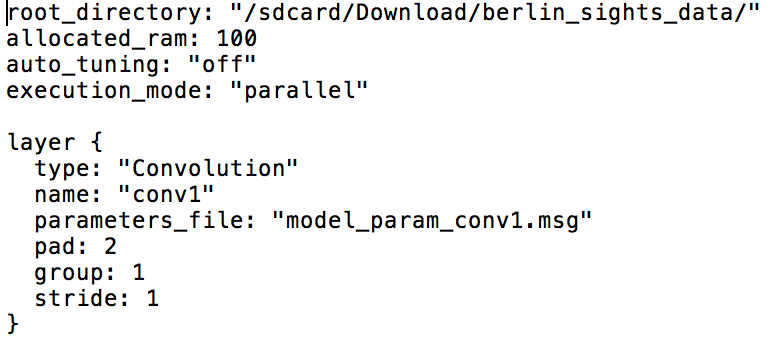
\includegraphics[width=0.5\textwidth]{def_file.png}
  \caption{Excerpt of a CNNDroid definition file}
  \label{fig:def_file}
\end{figure}

Not essential for the execution of CNNDroid, but very helpful for processing the final results, is a labels file. This file should specify human-readable names for the extractable classes. The order inside this file should be mapped to the output order of the last layer (probably a fully-connected layer), i.e. the first value of the output array should correspond to the first class name inside the labels file. The class names should be newline-separated.

\subsection{Training the model}
We trained our deep learning model based on crawled images with the caffe framework. The training occurred on an HPI server (accessible under the IP 172.16.18.178 and username msws2016t1). Caffe is already installed there and a variety of crawled images, as well as a labels file with the paths to each image are available inside the \texttt{training\_data} folder. Inside the same folder you can also find the \texttt{training\_full.sh} script, which can be executed to start the training and create a model.\\
An example model can be found in the \texttt{training\_data/berlin\_sights\_model} folder.\\
In order to test the model quickly, caffe provides an ipython notebook on their Github repository. This repository is checked out in the \texttt{caffe} folder. To start the notebook an ssh-tunnel has to be created to your local machine, e.g. using\\\\
\texttt{ssh -N -f -L localhost:8888:localhost:8889 msws2016t1@172.16.18.178}\\\\
Using a normal ssh connection to the server, the notebook can be executed with the command\\\\
\texttt{ipython notebook --no-browser --port=8889}\\\\
and viewed in a webbrowser on the local machine under the address \texttt{localhost:8888}.\\
The notebook itself provides possibilities to classify an image downloaded from a web address, view the output of specific layers and more.

\subsection{Convert Trained Models into CNNDroid-compatible Format}
As mentioned before, CNNDroid uses a format called MessagePack for the layer definitions. MessagePack is a binary serialization format for exchanging data, comparable to JSON\footnote{JavaScript Object Notation}, but other than JSON it is not human-readable. The omission of this constraint makes it possible to reduce size and increase parsing speed of the data stored inside. This is especially important due to the limited storage that most smartphones posses, especially compared to big servers, where deep learning is usually executed.\\
Figure \ref{fig:json_vs_msgpack} illustrates how MessagePack saves storage space by using types (JSON encodes everything as strings, so for example, `true' uses four Bytes, while it only uses one Byte using MessagePack) and dropping control symbols, like the curly braces \{\}.

\begin{figure}[H]
  \centering
    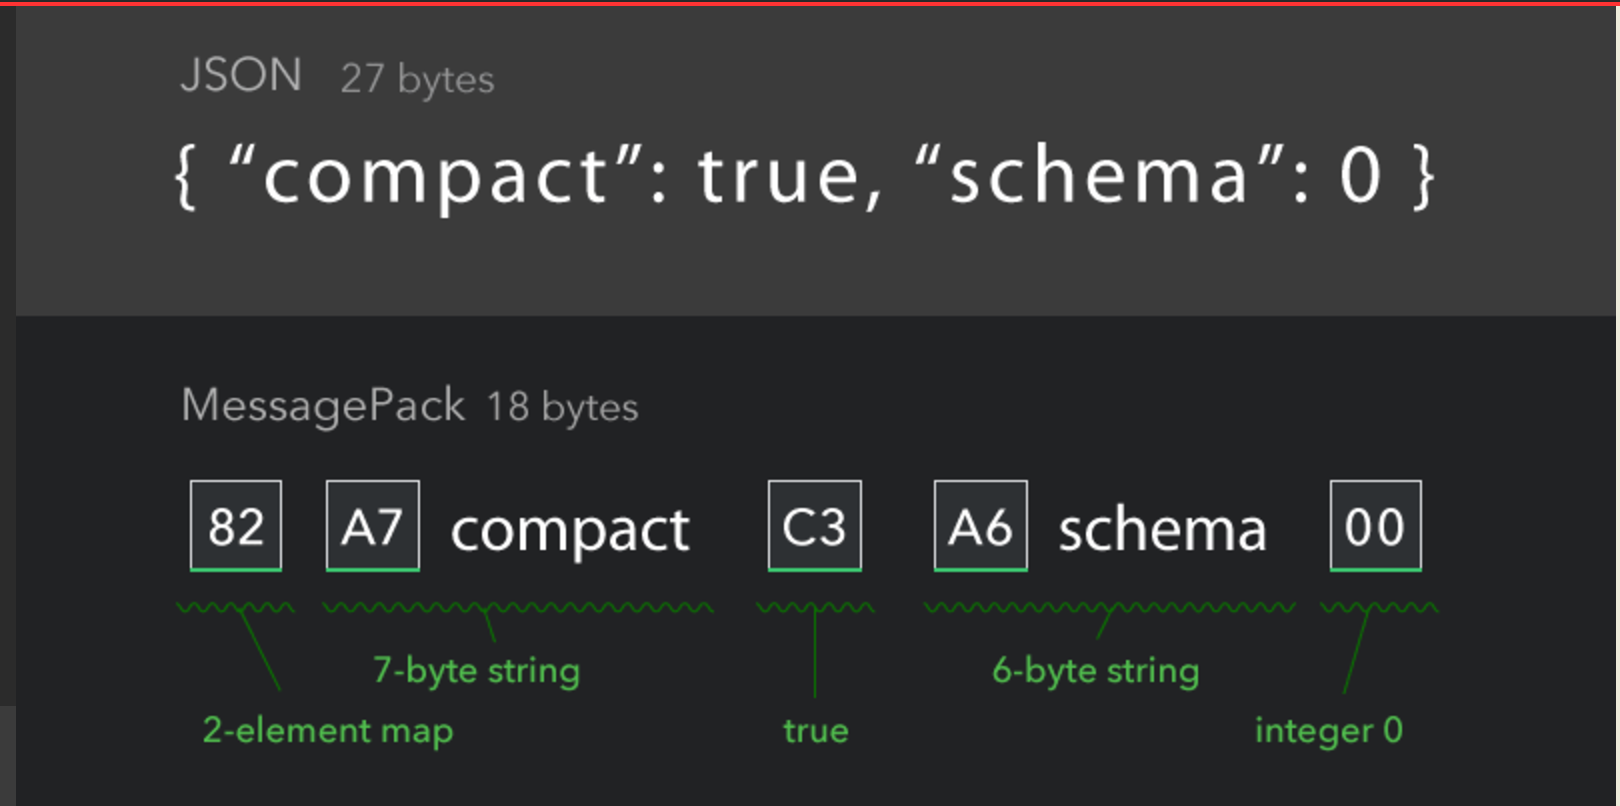
\includegraphics[width=0.5\textwidth]{json_vs_msgpack.png}
  \caption{Comparison JSON and MsgPack}
  \label{fig:json_vs_msgpack}
\end{figure}

In order to convert models from the aforementioned desktop/server deep learning frameworks, CNNDroid provides conversion scripts, which can be found in the\\
\texttt{CNNDroid/Parameter Generation Scripts/} folder. The script for Caffe is written in Python and requires the packages \lstinline[language=python]{numpy} and \lstinline[language=python]{msgpack} to be installed.\\
Three variables need to be defined.
\begin{itemize}
  \item{\texttt{MODEL\_FILE} - The absolute path to the trained model}
  \item{\texttt{MODEL\_NET} - The absolute path the deployment prototxt file, which specifies the parameters for the layers}
  \item{\texttt{SAVE\_TO} - The saving path}
\end{itemize}
The output are converted layer files in MessagePack format. The definition and label files have to be created manually. For the definition file, most of the content of the prototxt deployment file can be used. Only some parts of the syntax have to be adapted to a CNNDroid parsable format.\\
\newpage
\subsection{CPU vs GPU performance}
For a comparison of the sequential and parallel mode of CNNDroid we used the Android emulator using 2 GB of RAM. We used the berlin sights classifier, provided in the berlin\_sights\_data folder.

\begin{center}
  \begin{tabular}{l|c|r}
    layer & sequential time in ms & parallel time in ms \\\hline
    conv1 & 277 & 75\\
    pool1 & 22 & 47\\
    relu1 & 1 & 1\\
    conv2 & 299 & 27\\
    pool2 & 8 & 23\\
    conv3 & 161 & 24\\
    pool3 & 4 & 6\\
    ip1 & 1 & 5\\
    ip2 & 0 & 0\\
    prob & 0 & 0\\\hline
    sum & 773 & 208\\
  \end{tabular}
\end{center}

We can see that especially the more complicated convolutional layers profit from the additional speed of the GPU. Copying data from the RAM to GPU memory is usually very high, which is why the sequential mode can be faster for layers that do not do a lot of processing. In general, the parallel, GPU-accelerated processing speed is about three times faster than sequential, CPU-only processing.\\
The CNNDroid paper\cite{cnndroid2016} states a 12-times speedup with the CIFAR10 dataset on a Samsung Galaxy Note 4.\\
Our test machine was a MacBook Pro with an Intel Iris Graphics 6100 GPU and a 2.9 GHz Intel Core i5 CPU using the Android Studio emulator.\\
Apparently, the emulator does not reach such a significant overall speedup as the one stated in the paper. The \texttt{conv2} layer reaches an 11-times speedup, which comes close, but in sum it only reaches a third of the expected performance.\\
This however can potentially have a variety of reasons. Our testing setup does not follow lab conditions. It is not possible to know how the Android Studio emulator uses the MacBooks resources. Additional overhead is to be expected when communicating with the hardware. Also the CPU in the MacBook is more powerful than the one inside the Samsung phone (using an NVidia Jetson-style dual CPU consisting of one Quad-core 1.9 GHz Cortex-A57 and one Quad-core 1.3 GHz Cortex-A53, usually only using the A57 for high-computation tasks), which would decrease the speedup for the parallelized computation as the sequential computation is faster.\\
In theory the GPU of the MacBook should perform a lot better than the Samsung Galaxys GPU (which is capable of 48 parallel tasks, while the MacBooks GPU is capable of many hundred computations at the same time), it is however possible that the layer doesn't provide so many calculations, so that the full performance can not be used.\\
Overall, it is apparent, that the parallelization of the classification creates a clear speedup, which does however not reach that promised in the paper using our test setup.